\documentclass[]{article}
\usepackage[super,numbers]{natbib}

\usepackage{fullpage}
\usepackage{listings}
\usepackage{url}
\usepackage{authblk}
\usepackage{graphicx}
\usepackage{color}

\lstset{language=Python}

% local definitions
\newcommand{\sgcomment}[1]{{\textcolor{red}{SG: #1}}}
\newcommand{\bmhcomment}[1]{{\textcolor{blue}{BMH: #1}}}
\newcommand{\aprcomment}[1]{{\textcolor{magenta}{APR: #1}}}
\newcommand{\tdwcomment}[1]{{\textcolor{cyan}{TDW: #1}}}

% cross-reference with supplement
\usepackage{xr}
\externaldocument{supplement}

\begin{document}

\title{A weakly structured stem for human origins in Africa}
\author[1]{Aaron P. Ragsdale}
\author[2]{Timothy D. Weaver}
\author[3]{Elizabeth G. Atkinson}
\author[4]{Eileen Hoal}
\author[5]{Marlo M\"{o}ller}
\author[2,6,*]{Brenna M. Henn}
\author[7,**]{Simon Gravel}
\affil[1]{Department of Integrative Biology, University of Wisconsin, Madison, WI, USA}
\affil[2]{Department of Anthropology, University of California, Davis, Davis, CA, USA}
\affil[3]{FIXME: DSI-NRF Centre of Excellence for Biomedical Tuberculosis Research; South African Medical Research Council Centre for Tuberculosis Research; Division of Molecular Biology and Human Genetics, Faculty of Medicine and Health Sciences, Stellenbosch University, Cape Town, South Africa}
\affil[4]{FIXME}
\affil[5]{FIXME}
\affil[6]{UC Davis Genome Center, University of California, Davis, Davis, CA, USA}
\affil[7]{Department of Human Genetics, McGill University, Montreal, QC, Canada}
\affil[*]{bmhenn@ucdavis.edu}
\affil[**]{simon.gravel@mcgill.ca}
\maketitle

\abstract{
While a modern human origin within Africa is now broadly accepted, considerable
uncertainty surrounds specific models of divergence and migration across the
continent. Progress is hampered by a paucity of fossil and genomic data, as
well as variability in dating. Here we use linkage disequilibrium and
diversity-based statistics, optimized for rapid, complex demographic inference
to discriminate among such models. We infer detailed demographic models for
populations across Africa, including representatives from eastern and western
groups, as well as 44 newly whole-genome sequenced individuals from the Nama
(Khoe-San). Despite the complexity of African population history, present-day
population structure dates back to Marine Isotope Stage (MIS) 5. The earliest
population divergence among contemporary populations occurs 120-135ka, between
the Khoe-San and other groups. Prior to the divergence of contemporary African
groups, we infer long-lasting structure between two or more weakly
differentiated ancestral Homo spp. populations connected by gene flow over
hundreds of thousands of years (i.e. a weakly structured stem). We find that
weakly structured stem models provide more likely explanations of polymorphism
that had previously been attributed to contributions from archaic hominins in
Africa.
\sgcomment{IF we were not afraid of the racists, we could write something like:
"Despite the genetic similarity between these populations, 4 to 10\% of random
genetic differences among [modern human populations] can be attributed to this
early genetic drift.}
In contrast to models with archaic introgression, we predict that fossil
remains from coexisting ancestral populations should be morphologically
similar. We show that model misspecification explains variation in previous
divergence time estimates and argue that studying a suite of models is key to
robust inferences about deep history.
}

\section*{Introduction}

Archaeological sites from the Middle Stone Age (approx. 300ka-40ka) are widely
distributed across Africa, and are particularly well represented in the
northern, eastern and southern parts of the continent. Similarly, fossil crania
such as those from the sites of Jebel Irhoud \citep{Hublin2017-cq}, Herto
\citep{White2003-bk} and Klasies River \citep{Deacon1995-rx} demonstrate that
anatomically derived \emph{Homo sapiens} features were also present across the
continent during this period. It has been difficult to reconcile these lines of
evidence with evidence from genomics, which have suggested a predominantly
tree-like model of recent population divergence from a single ancestral
population. It is unclear whether fossil specimens and archaeological sites
represent populations which contributed to our ancestors as population
precedents, or were local “dead-ends” from which contemporary \emph{Homo
sapiens} do not descend. Recently, synthetic attempts to reconcile genetic and
paleoanthropological data include proposals for a Pan-African origin of
\emph{Homo sapiens} by which populations in many regions of the continent
contributed to the formation of Homo sapiens beginning at least 300ka
\citep{Stringer2016-mj,Scerri2018-nl,Scerri2019-xg}.

Genetic models have been hampered in their contribution to this discussion
because they primarily assume (or, at least, have been tested under) a
tree-like model of isolation-with-migration. Alternative theoretical scenarios
have been proposed, such as stepping stone models \citep{Arredondo2021-qa} or
population coalescence and fragmentation \citep{Scerri2019-xg}. These
approaches are more challenging to interpret and fit to data. However, new
population genetic inference tools now allow for inference involving tens to
hundreds of genomes from multiple populations and greater complexity
\citep{Kamm2020-vn,Ragsdale2019-nt,Speidel2019-nj}. Inspired by evidence for
Neanderthal admixture with modern humans in Eurasia, several recent articles
have shown that introducing an archaic ghost population contributing to African
populations in the period surrounding the Out-of-Africa migration event
substantially improves the description of genetic data relative to
single-origin models
\citep{Plagnol2006-lt,Hammer2011-bx,Hsieh2016-gk,Hey2018-pw,Ragsdale2019-nt,Durvasula2020-td,Lorente-Galdos2019-vz,Durvasula2020-td}.
This has driven speculation about the geographic range of this ghost
population, possible links to specific archaic remains, and the possibility of
finding ancient DNA evidence (e.g., \citet{Hsieh2016-gk}). However, these prior
articles share two weaknesses. First, they only contrast a single-origin model
with an archaic admixture model, leaving out other plausible models
(Figure~\ref{fig:supp-possible-models} and \citet{Henn2018-rf}). Second, they
focus on a small subset of African diversity, either because of small sample
sizes (2-5 genomes) or because they rely on 1000 Genomes data which only
recruited populations of recent West African ancestry. While ancient DNA from
Eurasia has helped us understand early human history outside of Africa, there
is no comparably ancient DNA to elucidate early history in Africa.

Here, we therefore aim to discriminate among a broader set of demographic
models by interrogating the genomes of contemporary populations. We take as our
starting point 4 classes of models (single population expansion, single
    population expansion with regional persistence, archaic admixture, and
multi-regional evolution, Figure~\ref{fig:supp-possible-models}), using 290
genomes from southern, eastern, and western Africa as well as Eurasia. By
including geographically and genetically diverse populations across Africa, we
infer demographic models that explain more aspects of genetic diversity in more
populations than previously reported. These analyses confirm the inadequacy of
tree-like models and provide an opportunity to directly evaluate a wide range
of alternative models.

\section*{Results}

We inferred detailed demographic histories using 4x-8x whole-genome sequencing
data for four diverse African populations, comprising the Nama (Khoe-San from
South Africa, newly presented here), Mende (MSL from Sierre Leone
\citep{1000_Genomes_Project_Consortium2015-zq}), Gumuz (recent descendents of a
hunter-gatherer group from Ethiopia \citep{Gurdasani2015-qy,Gopalan2019-wd}),
and Eastern African agriculturalists (Amhara and Oromo from Ethiopia
\citep{Gurdasani2015-qy}). The Amhara and Oromo populations, despite speaking
distinct Afro-Asiatic languages, are highly genetically similar
\citep{Pagani2015-pz,Gopalan2019-wd} and thus the two groups were combined for
a larger sample size (Figure~\ref{fig:1}). We also included the British
(GBR) from the 1000 Genomes Project in our demographic models as a
representative source of back-to-Africa gene flow and recent colonial admixture
in South Africa. Finally, we added a high-coverage ancient Neanderthal genome
from Vindija Cave, Croatia \citep{Prufer2017-kk} to account for archaic gene
flow from Neanderthals in non-Africans and gauge the relative time depth of
divergence, assuming Neanderthals diverged 550ka from a common stem. For each
population, we computed low-order allele frequency and linkage disequilibrium
(LD) statistics that are well suited for both low- and high-coverage genomes
\citep{Ragsdale2019-nt,Ragsdale2020-nz}. Using a maximum-likelihood inference
framework, we then fit to these statistics a family of parameterized
demographic models that involve population splits, size changes, continuous and
variable migration rates, and punctuated admixture events, to learn about the
nature of population structure over the past million years.

\begin{figure}[ht]
\begin{center}
\makebox[\textwidth][c]{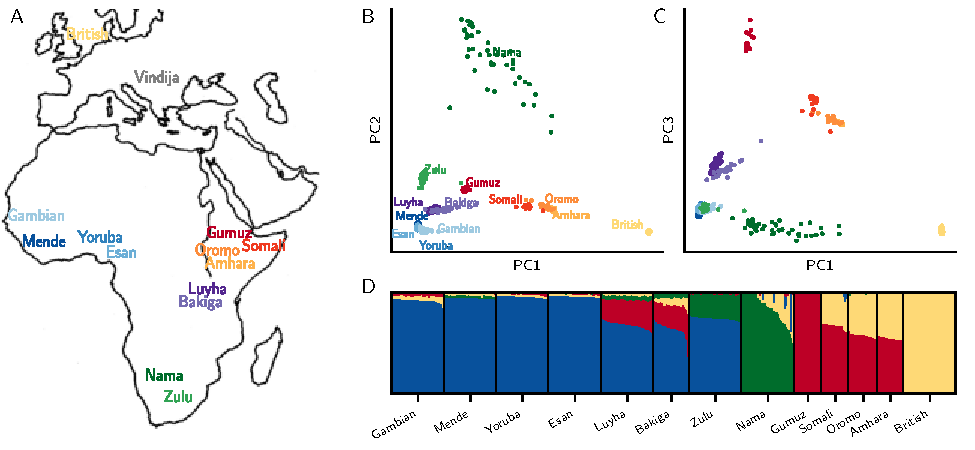
\includegraphics{figures/fig1.pdf}}
\caption{\textbf{Geography and genetic diversity within Africa}.
    \aprcomment{In the models presented below, we focus on the Nama, 
    Mende (MSL), Gumuz, and Oromo and Amhara.}
}
\label{fig:1}
\end{center}
\end{figure}

\subsection*{A Late Middle Stone Age common ancestry for contemporary humans}

We began with a model of geographic expansion from a single ancestral source
followed by migration between populations
(Figure~\ref{fig:supp-possible-models}A), without allowing for contribution
from an archaic African lineage. As expected \citep{Ragsdale2019-nt}, this
first model was a poor fit to the data qualitatively
(Figure~\ref{fig:supp-single-origin-fits}) and quantitatively (log-likelihood
($LL$) $\approx -189,000$, Table~\ref{tab:supp-single-origin}). We next explored a
suite of models in which population structure predates the differentiation of
contemporary groups, including models allowing for ancestral reticulation
(Figure~\ref{fig:supp-possible-models}B), archaic admixture
(Figure~\ref{fig:supp-possible-models}C), and African multi-regionalism
(Figure~\ref{fig:supp-possible-models}D).

Regardless of the model choice for early epochs, inference of recent human
demographic history from two thousand \aprcomment{why two thousand, instead of
just ``up to 150ka''?} to 150ka was remarkably robust. The earliest divergence
among contemporary sampled human populations differentiates the southern
African Nama from other African groups between 110--135ka, with low to moderate
levels of subsequent gene flow \aprcomment{(Table 1)}. In none of the
high-likelihood models which we explored did the divergence between Nama and
other populations exceed $\sim$150ka. We conclude that, regardless of model
specification, geographic patterns of \emph{Homo sapiens} population structure
date back to the Late Middle Stone Age in Africa, likely arising during MIS 5.
Although we find evidence for earlier population structure in Africa (see
below), present-day populations cannot be easily mapped onto these more ancient
stem groups as only a small proportion of drift between modern populations can
be attributed to drift between stems \aprcomment{(Figure 3)}. 

Given this consistency in inferred recent history and the numerical challenge
of optimizing a large number of parameters, we fixed several parameters related
to recent population history so as to focus on more ancient events (Supp.
Methods). The time of divergence of Western and Eastern African populations was
set to 60ka, just prior to the split of Eurasians and East Africans 50ka. Both
models predict relatively high subsequent gene flow between the two regions
($m=2\times10^{-4}$). Admixture from Neanderthals to Europeans directly
following the out-of-Africa migration was set to 1.5\% at 45kya (Supp.
Methods). Back-to-Africa gene flow at the beginning of the Holocene primarily
affected the ancestors of the Ethiopian agricultural populations, comprising
over half of their genetic ancestry, estimated to be 64--65\%. The past 5,000
years also saw major demographic changes, including strong population growth
for Western Africans as they specialized in yam and oil palm agriculture
(estimated 3-fold growth). We observe significant gene flow from the Amhara and
Oromo into the Nama, a signal which is likely a proxy for the movement of
Eastern African caprid and cattle pastoralists
\citep{Henn2008-xo,Breton2014-xb}, here estimated to constitute a 25\% ancestry
contribution 2,000 ya. Colonial period admixture from Europeans into the Nama
was estimated at 15\%, similar to proportions inferred by ADMIXTURE
\aprcomment{cite} (Figure~\ref{fig:1}).

\subsection*{Deep population structure but not archaic admixture within Africa}

\subsection*{Reconciling multiple lines of genetic evidence}

\section*{Discussion}

\subsection*{The Middle Stone Age in Africa}

\subsection*{Contrasting archaic admixture and a weakly structured stem}

\section*{Methods}
A placeholder citation \citep{Kelleher2016-lw}.

\begin{figure}[ht]
\begin{center}
\makebox[\textwidth][c]{} % 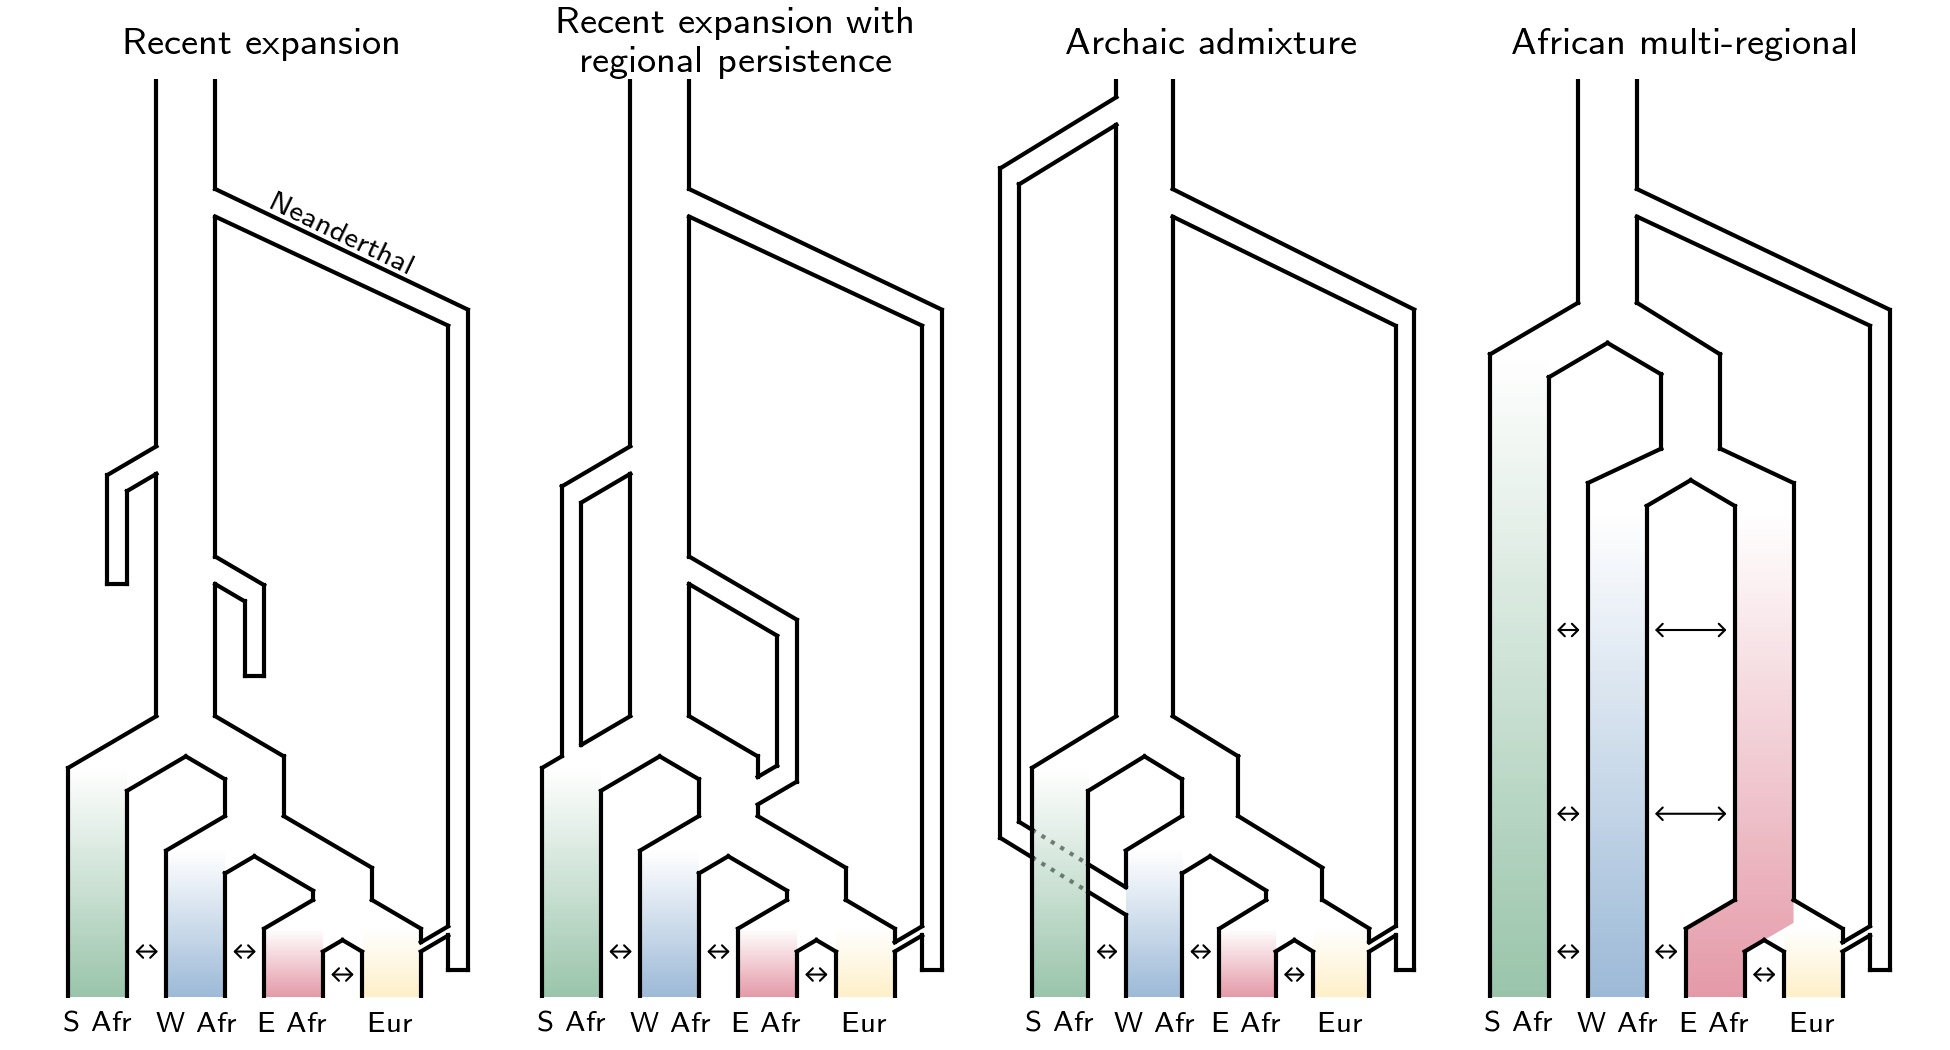
\includegraphics{figures/fig2.png}}
\caption{\textbf{The second main figure}.
    A placeholder - best fit model(s).
}
\label{fig:2}
\end{center}
\end{figure}

\begin{figure}[ht]
\begin{center}
    \makebox[\textwidth][c]{} % 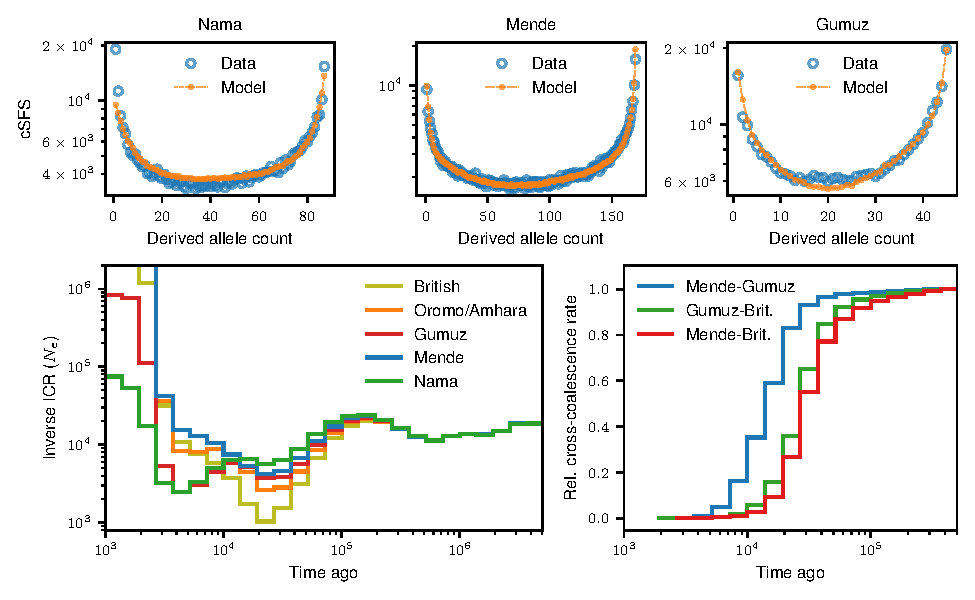
\includegraphics{figures/fig3.pdf}}
\caption{\textbf{The third main figure}.
    A placeholder - validation (Relate and cSFS).
}
\label{fig:3}
\end{center}
\end{figure}

\begin{figure}[ht]
\begin{center}
    \makebox[\textwidth][c]{} % 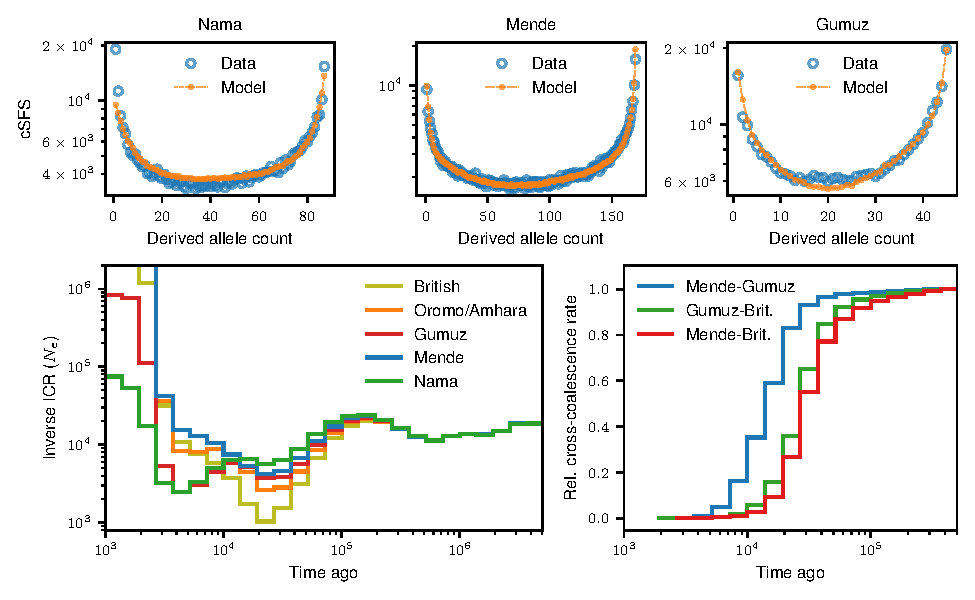
\includegraphics{figures/fig3.pdf}}
\caption{\textbf{The fourth main figure}.
    A placeholder - predictions (FST and/or f4).
}
\label{fig:4}
\end{center}
\end{figure}

\section*{Acknowledgements}

\break

\bibliographystyle{unsrtnat}
\bibliography{paper}
\end{document}
